\documentclass[a4paper, amsfonts, amssymb, amsmath, reprint, showkeys, nofootinbib, twoside]{revtex4-1}
\usepackage[english]{babel}
\usepackage[utf8]{inputenc}
\usepackage[colorinlistoftodos, color=green!40, prependcaption]{todonotes}
\usepackage[pdftex, pdftitle={Article}, pdfauthor={Author}]{hyperref} % For hyperlinks in the PDF
\usepackage{graphicx} % For figures
\usepackage{algorithm} % For algorithms
\usepackage{algpseudocode}

%\setlength{\marginparwidth}{2.5cm}
\bibliographystyle{apsrev4-1}
\begin{document}
\title{Self-Organization in the Minority Game}

\author{Gaëtan Ecrepont}
    \email[]{gaetan.ecrepont@polytechnique.edu}
    \affiliation{ENS Paris-Saclay, FRANCE}
\author{Guillaume Martin-Festa}
    \email[]{guillaume.martin-festa@polytechnique.edu}
    \affiliation{ENS Paris-Saclay, FRANCE}

\date{\today} % Leave empty to omit a date

\begin{abstract}
    abstract abstract abstract abstract abstract abstract abstract abstract abstract abstract abstract abstract abstract abstract abstract abstract abstract abstract abstract abstract abstract abstract abstract abstract abstract abstract abstract abstract abstract abstract abstract abstract abstract 
\end{abstract}


\maketitle


\section{Introduction}
\label{sec:introduction}

\subsection{El Farol Bar Problem}
A key concept in the minority game is *inductive thinking*, which can be roughly described as the ability to learn from the past to make inferences about the future. It is very different from *deductive thinking*, which amounts to applying a predefined set of rules to a given situation. A good introduction to inductive thinking is the *El Farol Bar Problem* \cite{Arthur_1994}, which we present in this section.

The problem is simple: every Thursday, 100 people consider visiting the El Farol Bar, but the venue is enjoyable only if attendance stays below 60. If too many go, the bar is overcrowded; if too few go, those who stayed home may regret missing out. Without direct communication, individuals must predict attendance based on past data. If their forecast suggests a crowded bar, they stay home; otherwise, they go. Every night, individuals make their decision independently, and the bar's attendance fluctuates based on their choices.

To win this game, one needs to be in the minority. Crucially, there is no single optimal strategy since the best decision depends on the decisions of others. This is a key feature of the game: agents must adapt to the behavior of others, leading to complex dynamics. The game is played repeatedly, and agents can learn from past experiences to improve their predictions.

To simulate this game using agent-based modelling, Arthur proposed that each agent uses a fixed set of simple forecasting rules (e.g. assuming attendance will be the same as last week or averaging past values). Over time, agents favor rules that perform well, adjusting their choices accordingly. Remarkably, Arthur's simulations showed that *attendance naturally fluctuates around the optimal level of 60*, despite the absence of central coordination. This *self-organizing* behavior emerges from agents adapting to each other’s strategies.

There is more to be said about the El Farol Bar Problem, but we will not go into details here. The key result is that inductive thinking can lead to self-organization. We will now pass to the *Minority Game*, which is a generalization of the El Farol Bar Problem that is more amenable to mathematical analysis.


\subsection{The Minority Game}

The El Farol Bar Problem directly inspired the Minority Game, a simple model introduced by Challet and Zhang \cite{Challet_1997} to study self-organization in a binary game.

In the Minority Game, an odd number of agents repeatedly choose between two options (e.g., A or B, buy or sell, go or stay, etc.) The goal is to be in the minority group\footnote{There is always a strict minority since the number of agents is odd.}. The game is played in identical rounds, and each agent has a fixed individual set of strategies to choose from. These strategies can be thought of as simple rules or heuristics that guide the agents' decisions based on past outcomes. At the end of each round, the agents receive a reward or penalty based on their choices. The agents in the minority (those who chose the less popular option) are rewarded, while those in the majority (those who chose the more popular option) are penalized.

Just like the El Farol bar problem, this is a negative sum game since by definition only the minority wins at each round. Ideally, agents would coordinate so that the minority is a large as it can be (i.e. half the population). And indeed computer simulations show that the game naturally self-organizes to a state where the number of agents in the minority is close to half the population.


\section{Presentation of the system}
\label{sec:presentation}

We now formally introduce the model. We first recall the mathematical framework of the Minority Game, and then we present the dynamics of the system. We will go quickly, and for more details we refer the reader to the original paper by Challet and Zhang \cite{Challet_1997}.

\subsection{Theoretical framework}

Throughout the rest of the paper, we will use the following notations:
\begin{itemize}
    \item $N$: number of agents
    \item $S$: number of strategies per agent
    \item $M$: memory length of each
    \item $s_i(t)$: strategy of agent $i$ at time $t$
    \item $S_i$: set of strategies of agent $i$
    \item $a_i(t) = \pm 1$: action of agent $i$ at time $t$
    \item $A(t) = \sum_{i=1}^N a_i(t)$: aggregate movement of the population at time $t$, also called "attendance", in analogy with the El Farol Bar Problem
    \item $a(t) = \pm 1$: action of the population at time $t$, defined as $a(t) = \text{sign}(A(t))$
\end{itemize}

The game has $N$ agents, each with memory length $M$. The game's history is represented by binary string $H$ which is initially a $M$-long string of random bits and to which we append at the end of each step a "0" bit (resp. a "1" bit) when the action $a(t)$ is $-1$ (resp. $+1$).

At a given time $t$, agents base their action $a_i(t)$ on the last $M$ values in the game's history, i.e. on the state $\mu(t) = (H[t-M], \ldots, H[t-1])$. The state $\mu(t)$ is a binary string of length $M$ that encodes the last $M$ actions of the population. Each agent has a set of $S$ strategies, which are mappings $\{0, 1\}^M \to \{-1, +1\}$ that determine the agent's action based on the current state $\mu(t)$.

At each turn $t$, each agent $i$ picks amongs its strategies $S_i$ the strategy $s_i(t)$ which has been the fittest so far\footnote{If there are several maxima, we sample one of them uniformly at random}. The fitness of a strategy is defined as the number of times it has been in the minority so far, i.e. the number of times $F_s(t) = \sum_{t' < t} \mathbb{1}_{s(\mu(t')) = -a(t')}$. The agent then plays the action $a_i(t) = s_i(t)(\mu(t))$. Once all agents have picked their action\footnote{Note that the order of play is irrelevant since the attendance is the same regardless of the order.}, the population's action is computed as $a(t) = \text{sign}(A(t))$. Finally, each player updates the fitness of all its strategies, as if it had played all of them\footnote{In some variants of the Minority Game, agents take into account their impact by giving an extra fitness reward to the strategy which they actually played. Interestingly, accounting for self-impact in this simple way removes many of the emergent phenomena of the game.}. Finally, the history is updated by appending the action of the population $a(t)$ to the history $H$.

The above set of rules can be summarized by the following algorithm:
\begin{algorithm}
    \caption{Minority Game}
    \label{alg:minority-game}
    \begin{algorithmic}[1]
        \State Initialize $H \sim U(\{0, 1\} ^M)$
        \For{$t = 0$ to $T$}
            \State $\mu(t) = H[t-M:t]$
            \For{$i = 1$ to $N$}
                \State $s_i(t) = \arg\max_{s \in S_i} F_s(t)$
                \State $a_i(t) = s_i(t)(\mu(t))$
            \EndFor
            \State $A(t) = \sum_{i=1}^N a_i(t)$
            \State $a(t) = \text{sign}(A(t))$
            \For{$i = 1$ to $N$}
                \For{$s \in S_i$}
                    \State $F_s(t+1) = F_s(t) + \mathbf{1}_ {s(\mu(t)) = -a(t)}$
                \EndFor
            \EndFor
            \State $H \gets H \cup \{a(t)\}$
        \EndFor
    \end{algorithmic}
\end{algorithm}


\subsection{Dynamics}
For the sake of simplicity and like many authors \cite{Challet_1997}, we will assume that $S=2$ i.e. agents only have two strategies, which we will denote $s_{i,+}$ and $s_{i,-}$ for convenience. We then introduce the following useful notations:
\begin{itemize}
    \item $D_i(t) = \frac{1}{2}\big(F_{s_{i,+}}(t) - F_{s_{i,-}}(t)\big)$: difference of fitness between the two strategies of agent $i$ at time $t$
    \item $a_{i,+}^\mu = a_{i,+}(\mu) = \pm 1$: action of agent $i$ when playing strategy $s_{i,+}$ and the game's state is $\mu$. We define $a_{i,-}^\mu$ similarly.
    \item $\omega_i^\mu = \frac{1}{2}\big(a_{i,+}^\mu + a_{i,-}^\mu\big)$
    \item $\xi_i^\mu = \frac{1}{2}\big(a_{i,+}^\mu - a_{i,-}^\mu\big)$
    \item $\Omega^\mu = \frac{1}{N} \sum_{i=1}^N \omega_i^\mu$: average of $\omega_i^\mu$ over the population. Can be thought of as the polarization of the system in state $\mu$.
\end{itemize}

Using those notations, note that the strategy ($s_{i,+}$ or $s_{i,-}$) played by agent $i$ at time $t$ is given by the sign of $D_i(t)$, i.e.
\begin{equation}
\label{eq:strategy}
    s_i(t) = \text{sign}(D_i(t))
\end{equation}
Consequently, the action of agent $i$ at time $t$ is given by:
\begin{equation}
    a_i(t) = a_{i,s_i(t)}(\mu(t)) = \omega_i^{\mu(t)} + s_i(t) \xi_i^{\mu(t)}
\end{equation}
From which we can deduce the attendance:
\begin{equation}
    A(t) = \sum_{i=1}^N a_i(t) = \sum_{i=1}^N \omega_i^{\mu(t)} + \sum_{i=1}^N s_i(t) \xi_i^{\mu(t)} = \Omega^{\mu(t)} + \sum_{i=1}^N s_i(t) \xi_i^{\mu(t)}
\end{equation}
The difference of fitness thus evolves according to the following equation:
\begin{equation}
\label{eq:difference}
    D_i(t+1) = D_i(t) - \xi_i^{\mu(t)} \textnormal{sign }A(t)
\end{equation}
Combining \eqref{eq:strategy} and \eqref{eq:difference}, we can see that the dynamics of the system is governed by the following equation:
\begin{equation}
\label{eq:dynamics}
    D_i(t+1) = D_i(t) - \xi_i^{\mu(t)} \textnormal{sign }\bigg(\Omega^{\mu(t)} + \sum_{j=1}^N s_j(t) \xi_j^{\mu(t)}\bigg)
\end{equation}


\section{Self-organization}
\label{sec:self-organization}

\subsection{Volatility}

\begin{figure}[H]
    \centering
    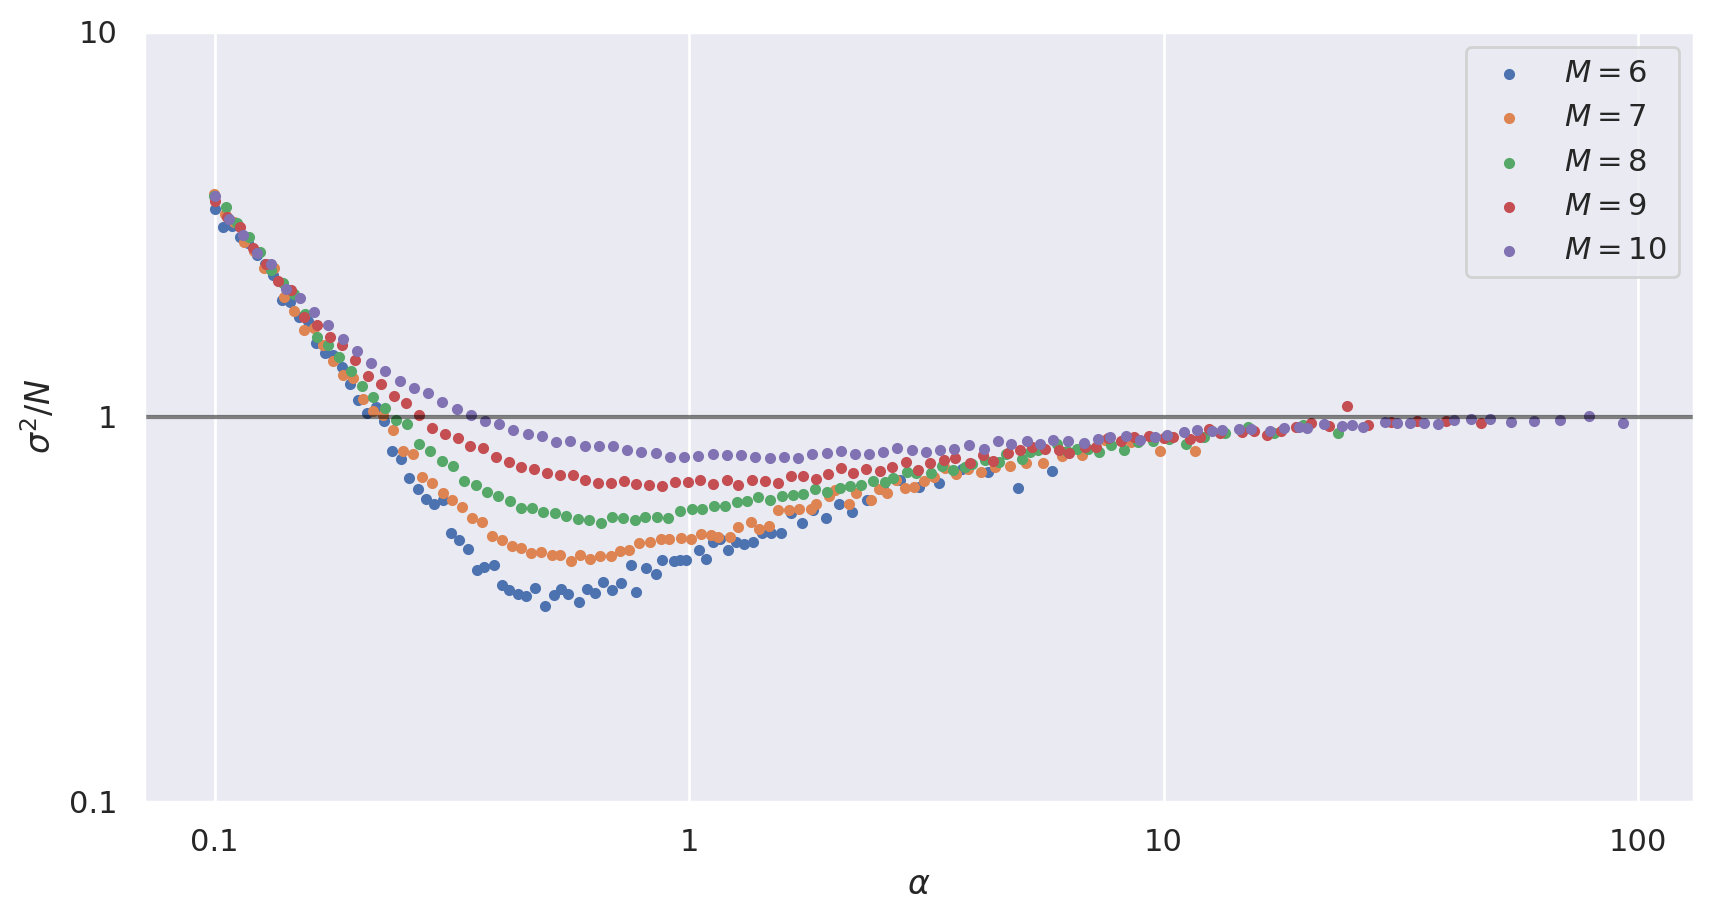
\includegraphics[width=0.42\textwidth]{figures/volatility.png}
    \caption{Long-term volatility of the system as a function of the parameter $\alpha = \frac{2^M}{N}$ for various couples $(N, M)$}
    \label{fig:volatility}
\end{figure}    

The horizontal line $\sigma^2=N$ corresponds to the case where agents are completely random. Note that the system self-organizes whenever $\alpha > \alpha_c \simeq 0.4$. On the contrary, when...

\subsection{Predictability}

\begin{figure}[H]
    \centering
    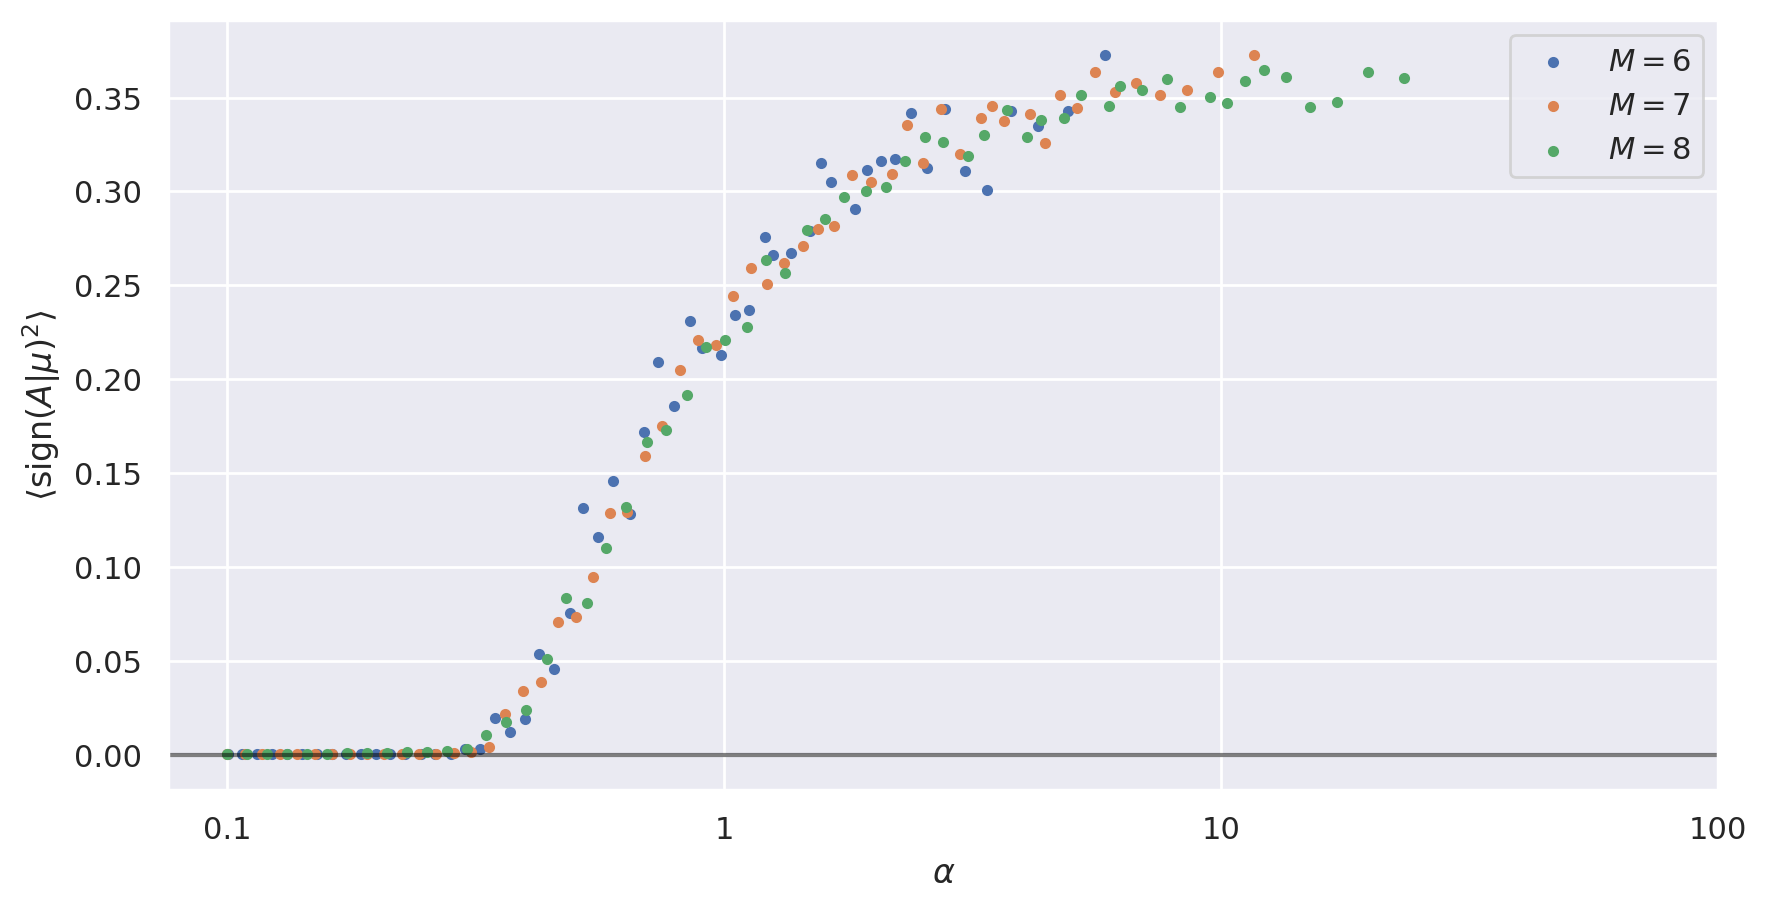
\includegraphics[width=0.42\textwidth]{figures/predictability.png}
    \caption{Predictability of the system as a function as a function of the parameter $\alpha = \frac{2^M}{N}$ for various couples $(N, M)$.}
    \label{fig:predictability}
\end{figure}


\bibliography{refs} % Entries are in the refs.bib file


\end{document}
